\section{Minimal Structure: SSO}


\subsection{Why Two Layers Emerge: Grounding in Bio-IFGT}

本節に入る前に、一点を固定しておく。

高速層と低速層という二層構造は、本稿が意識を説明するために便宜的に設けた区別ではない。この構造は、生命アトラクタの成立過程から必然的に現れる。

Bio-IFGT では、生命を「情報流が作る動的準閉包構造」として記述する。生命が環境との差を維持しながら自己を持続させるためには、少なくとも二つの異なる時間スケールの処理が必要になる。

第一は、即時的な環境応答を担う高速処理である。これは外部変化への予測・反応・誤差修正に関わり、揮発的で速い。

第二は、成功した反応条件を次の世代または次の状態へ保持するための低速処理である。これは沈殿的・安定的であり、一度刻まれた構造は簡単には崩れない。

Bio-IFGT のシミュレーション実験では、階層的な創発経路
$M \rightarrow \mathcal{I} \rightarrow N \rightarrow B \rightarrow E$
（morphogen field $\rightarrow$ information density $\rightarrow$ neural commitment $\rightarrow$ boundary stabilization $\rightarrow$ eye-like commitment）を辿る過程で、情報流による構造化が進むにつれて、高速な探索流と低速な安定化構造が自発的に分化することが確認されている。この二種の時間スケールは、完全に同期することも完全に分離することもなく、差を保ったまま共存する。

これは偶然の並存ではない。VED の観点では、完全閉包が通常状態として実現されない差の持続が構造を生み出す駆動力であり、二層の時間差こそがその駆動力の生物的実装である。

したがって、本稿が意識の最小時間構造として SSO を導入するとき、それはこの生命的二層分化の上に立っている。意識は生命アトラクタの外部に突然現れる現象ではなく、生命が高速応答と低速保持の差を維持し続けた結果として、その差が参照関係を開くようになった状態である。

この積み上げを踏まえた上で、以下では SSO を意識が成立するための最小時間構造として形式化する。

SSO は Speed-Scale Orchestration を指す。

これは、複数の時間スケールをもつ処理層が、中央制御なしに調整される構造である。

本稿では、SSO を意識が成立するための最小時間構造として扱う。

ここで重要なのは、SSO が脳の特定部位を指すものではないという点である。

SSO は解剖学的構造ではない。

それは、異なる速度で走る処理が、同期に潰れず、分離にも至らず、相互に干渉し続けるための時間的配置である。

\subsection{Two Minimal Layers}

最小構成として、ここでは少なくとも二つの処理層を考える。

第一に、高速層がある。

高速層は、予測、前方モデル、瞬間的な状態更新、即時反応に関わる。

この層の処理は速く、揮発的であり、多くはそのまま消えていく。

第二に、低速層がある。

低速層は、保存、統合、記憶沈殿、長期的構造変化に関わる。

この層の処理は遅く、安定的であり、一度沈殿したログは再参照可能な構造として残る。

この二つの層は、能力差を表しているのではない。

高速層が高級で、低速層が低級なのではない。

両者の違いは、向いている時間方向にある。

高速層は未来へ先行し、低速層は過去を保持する。

\subsection{Speed Differential}

SSO の最小条件は、二つの層が同じ速度で走っていないことである。

高速層の速度を $v_f$、低速層の速度を $v_s$ とすると、速度差は次のように表される。

\begin{equation}
\Delta v = v_f - v_s
\end{equation}

この速度差は、誤差ではない。

むしろ、SSO が成立するための条件である。

もし $\Delta v = 0$ なら、高速層と低速層は完全に同期し、両者の間に境界は生じない。

境界がなければ、現在処理と過去ログのあいだに参照関係は開かれない。

したがって、意識状態が成立するためには、少なくとも次の条件が必要になる。

\begin{equation}
\Delta v \neq 0
\end{equation}

ただし、速度差が大きければよいわけではない。

速度差が大きすぎれば、両層の対応は失われ、ログ参照は断片化する。

SSO に必要なのは、消えないが破綻もしない有限の速度差である。

\cref{fig:sso-ja} は、SSO の最小構造をまとめたものである。

\begin{figure}[H]
\centering
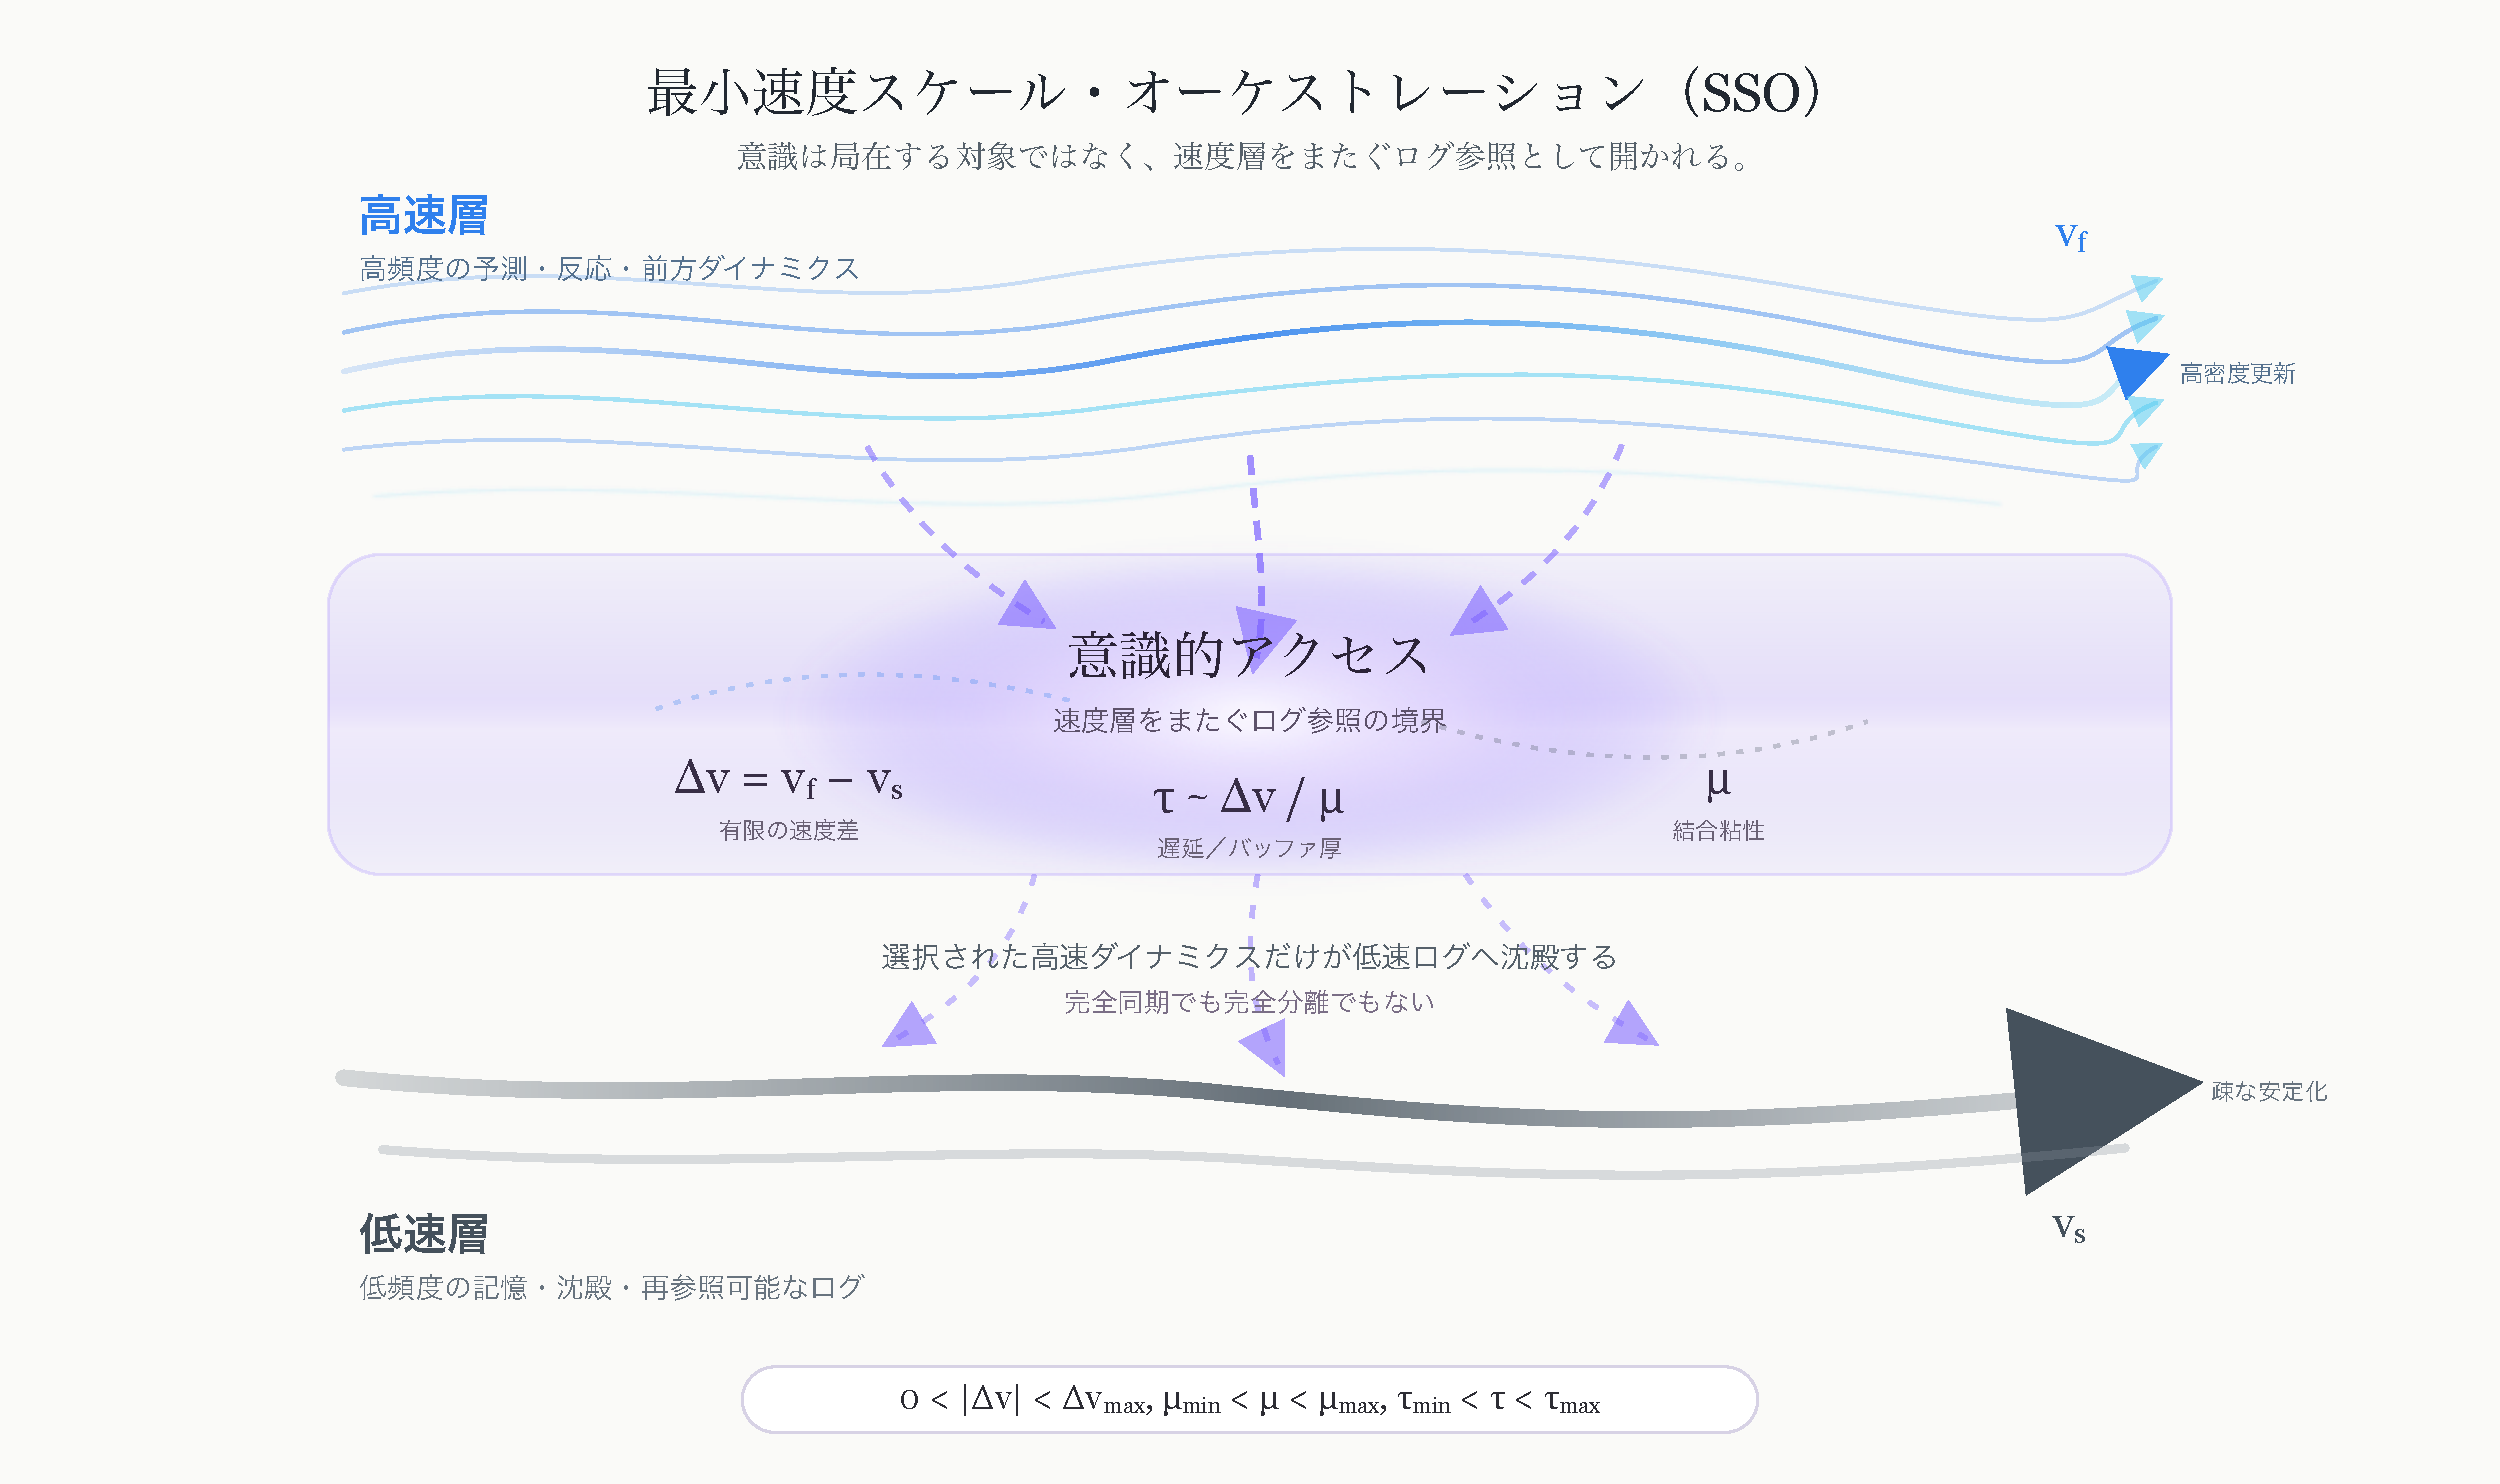
\includegraphics[width=0.92\linewidth]{figures_ja/figure1_sso_density_jp.pdf}
\caption{
Speed-Scale Orchestration（SSO）の最小構造。
意識は高速層または低速層のどちらか一方に局在するのではなく、高速な予測ダイナミクスと低速な沈殿ログが、有限の速度差、遅延、結合粘性のもとで相互参照可能になる境界に開かれる。
}
\label{fig:sso-ja}
\end{figure}

\subsection{Orchestration Without Control}

SSO において、処理層を統括する中央制御者は仮定されない。

高速層が低速層を支配するのでもなく、低速層が高速層を上から制御するのでもない。

両者は、それぞれの時間スケールで独立に走りながら、局所的に干渉する。

ここでいう orchestration とは、指揮者による制御ではない。

それは、異なる速度で走る処理が、互いの差を保ちながら、破綻しない範囲で結合することを意味する。

したがって、SSO は control ではなく coordination である。

より正確には、時間的非同期を完全には解消せず、その非同期を利用可能な構造として保持することである。

\subsection{Gate of Plasticity}

高速層と低速層の相互作用には、可塑性ゲートが必要である。

可塑性ゲートは、何を処理するかを決めるものではない。

それは、高速層の活動が低速層を変更できるかどうか、また低速層の構造が将来の高速過程をどの程度制約するかを調整する。

高速層の活動がすべて低速層へ書き込まれるなら、システムは過剰に硬直する。

逆に、高速層の活動がまったく低速層へ届かなければ、経験は沈殿せず、ログ参照は成立しない。

したがって、可塑性ゲートは開閉のスイッチではない。

それは、速度差、遅延、粘性を伴う時間的な通過条件である。

この通過条件によって、高速な処理の一部だけが低速層へ沈殿し、再参照可能なログとなる。

\subsection{Internal Delay and Buffering}

SSO において、遅延は欠陥ではない。

むしろ、遅延があるからこそ、現在処理と過去ログのあいだに参照可能な厚みが生まれる。

この内部遅延を $\tau$ と表す。

\begin{equation}
\tau \propto \frac{\Delta v}{\mu}
\end{equation}

ここで $\mu$ は、高速層と低速層の結合粘性を表す。

$\tau$ は主観的時間そのものではない。

それは、高速層で生じた処理が低速層へ沈殿し、ログとして参照可能になるまでの内部的な時間バッファである。

$\tau$ が小さすぎれば、処理は即時反応として流れ去り、参照可能なログになりにくい。

$\tau$ が大きすぎれば、現在処理とログ沈殿の対応が崩れ、意識状態は断片化する。

したがって、SSO は単に速い処理と遅い処理の並存ではない。

それは、適切な遅延幅を保持する構造である。

\subsection{SSO as Temporal Non-Closure}

VED の観点から見ると、SSO は時間的非閉包構造である。

高速層と低速層は、閉じようとする。

すなわち、処理は安定化し、沈殿し、ログとして固定されようとする。

しかし、完全に閉じてしまえば、速度差は消え、流れは止まり、意識の境界は失われる。

逆に、閉じなければ、処理は流れ去り、ログとして残らない。

SSO は、この二つの極のあいだにある。

閉じようとするが、閉じ切らない。

分離しようとするが、切れ切らない。

この非閉包的な時間構造の中で、現在処理と過去ログのあいだに参照関係が開かれる。

この意味で、SSO は意識を生成する装置ではない。

SSO は、意識が開かれうる時間的条件である。

\begin{quote}
\textbf{CT との対応（Conceptual Topography §2.4）：} 概念地形論では、低速層が形成する$\Phi$の地形は「意識の閾値以下で動く不可視のGPU」として記述される。思考は地形の上を流れるが、地形そのものは意識から直接参照されない。本稿の低速層／高速層の差が、CTではこの「可視の流れ（$J_I$）と不可視の地形（$\Phi$）の非対称性」として現れる。CTを読んだ後でこの節に戻ると、SSO の時間条件が概念地形の形成条件と同一の構造を持つことが見えてくる。
\end{quote}

\subsection{From SSO to Self-Sustaining Observer}

SSO は、Speed-Scale Orchestration として導入された。

しかし、この構造が安定した時間ループを形成するとき、同じ構造は Self-Sustaining Observer として読まれうる。

ここで observer とは、世界を眺める主体を意味しない。

それは、現在処理、過去ログ、可塑性ゲートが相互に閉じ切らないループを形成し、自己維持的に参照状態を保つ構造を指す。

高速層は未来を先取りする。

低速層は過去を保持する。

可塑性ゲートは、その両者の間で何が沈殿し、何が流れ去るかを調整する。

このループが安定したとき、システムは外部から制御されなくても、自己のログを参照しながら状態を更新できる。

ここに、観測者らしさが現れる。

ただし、それは主体が追加されたからではない。

時間構造が自己維持的になっただけである。

\subsection{Minimal Conditions}

以上をまとめると、SSO が成立するための最小条件は次のように整理できる。

\begin{enumerate}
\item 高速層と低速層が存在すること。
\item 両者のあいだに有限の速度差 $\Delta v$ があること。
\item 速度差が完全同期にも完全分離にも至らないこと。
\item 可塑性ゲートによって、処理の一部が低速層へ沈殿しうること。
\item 内部遅延 $\tau$ が、参照可能な時間的厚みとして保持されること。
\item この構造が中央制御なしに自己維持的ループを形成すること。
\end{enumerate}

この条件が満たされるとき、システムは単なる処理装置ではなく、ログ参照可能な時間構造を持つ。

この構造そのものは、まだ意識ではない。

しかし、この構造がなければ、意識は成立しない。

次節では、この SSO の内部で速度差を破綻なく変換する機構として、トルクコンバータ・アテンションを導入する。
